% !TEX root = ./final_report.tex

\begin{figure}
        \centering
        \begin{subfigure}[b]{0.3\textwidth}
                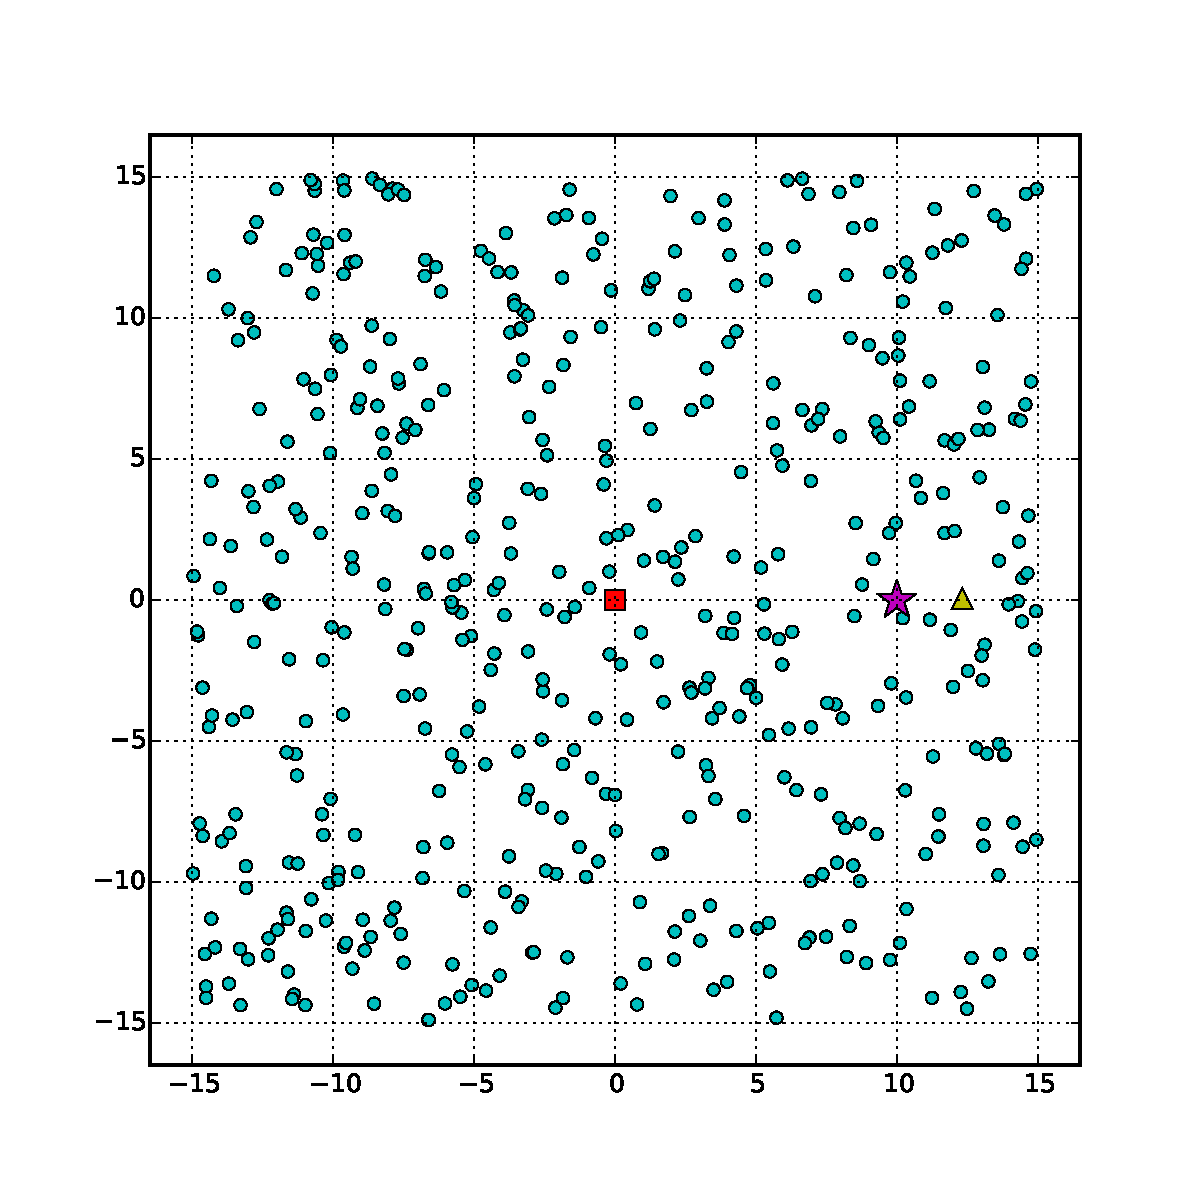
\includegraphics[width=\textwidth]{bad_range_initial}
                \caption{Initial belief state}
                \label{fig:bad_range_init}
        \end{subfigure}%
        ~ %add desired spacing between images, e. g. ~, \quad, \qquad, \hfill etc.
          %(or a blank line to force the subfigure onto a new line)
        \begin{subfigure}[b]{0.3\textwidth}
                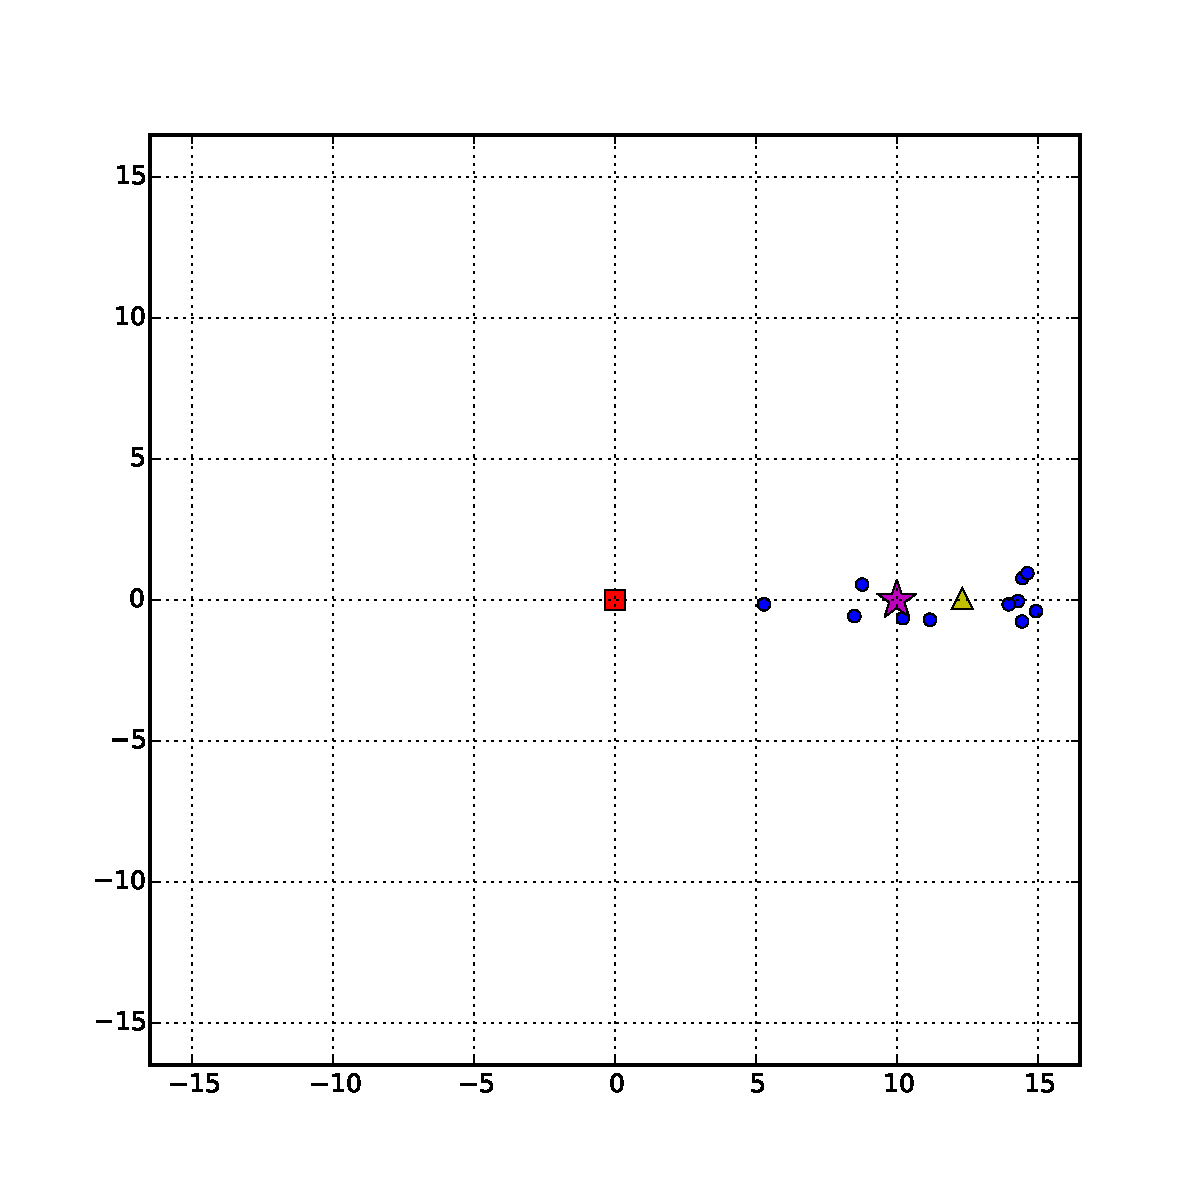
\includegraphics[width=\textwidth]{bad_range_first_obs}
                \caption{t=0, first observation}
                \label{fig:bad_range_t_0}
        \end{subfigure}
        ~ %add desired spacing between images, e. g. ~, \quad, \qquad, \hfill etc.
          %(or a blank line to force the subfigure onto a new line)
        \begin{subfigure}[b]{0.3\textwidth}
                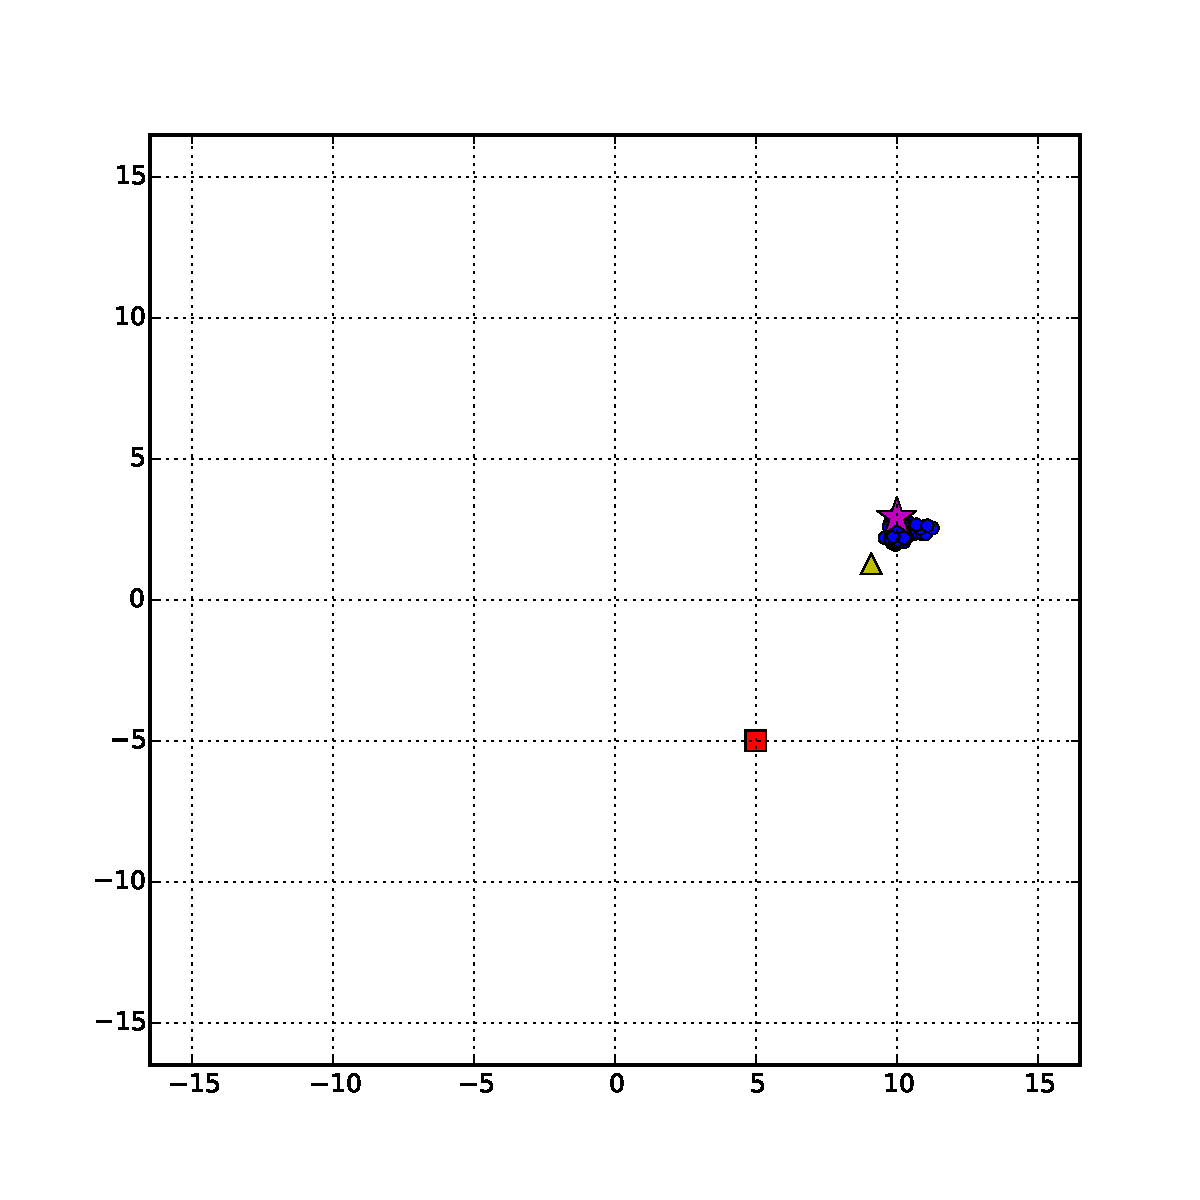
\includegraphics[width=\textwidth]{bad_range_t_2}
                \caption{t=2}
                \label{fig:bad_range_t_2}
        \end{subfigure}
        \begin{subfigure}[b]{0.3\textwidth}
                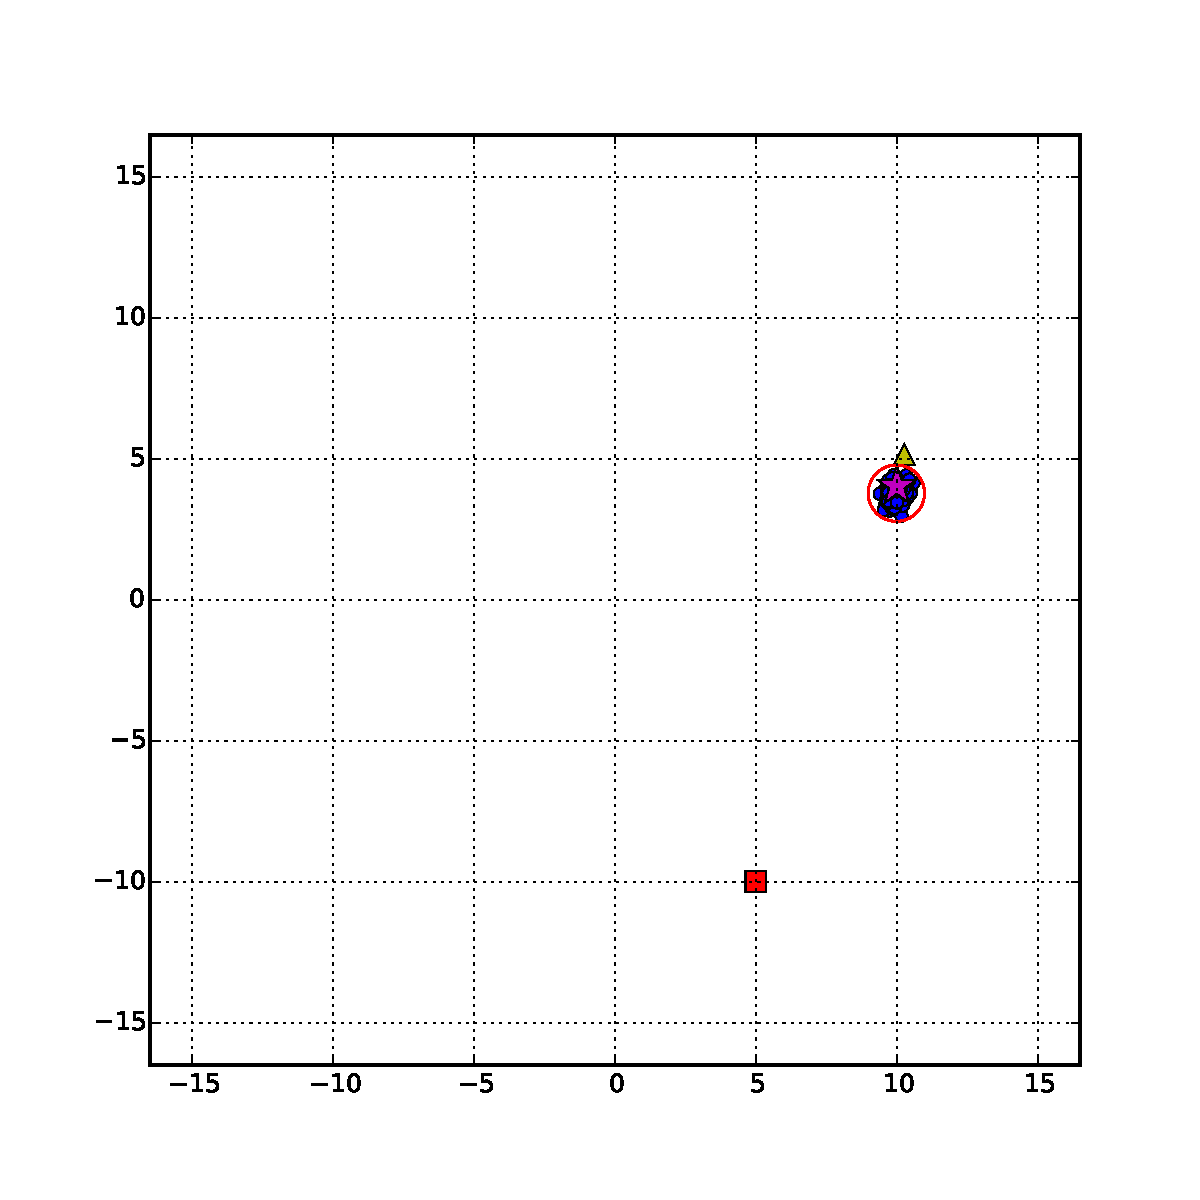
\includegraphics[width=\textwidth]{bad_range_t_3}
                \caption{t=3, agent engages target}
                \label{fig:bad_range_t_3}
        \end{subfigure}
        \caption{Bad range}\label{fig:bad_range}
\end{figure}